\documentclass{article} % For LaTeX2e
\usepackage{nips14submit_e,times}
\usepackage{amsmath}
\usepackage{amsthm}
\usepackage{amssymb}
\usepackage{mathtools}
\usepackage{hyperref}
\usepackage{url}
\usepackage{algorithm}
\usepackage[noend]{algpseudocode}
%\documentstyle[nips14submit_09,times,art10]{article} % For LaTeX 2.09

\usepackage{graphicx}
\usepackage{caption}
\usepackage{subcaption}

\def\eQb#1\eQe{\begin{eqnarray*}#1\end{eqnarray*}}
\def\eQnb#1\eQne{\begin{eqnarray}#1\end{eqnarray}}
\providecommand{\e}[1]{\ensuremath{\times 10^{#1}}}
\providecommand{\pb}[0]{\pagebreak}

\newcommand{\E}{\mathrm{E}}
\newcommand{\Var}{\mathrm{Var}}
\newcommand{\Cov}{\mathrm{Cov}}

\def\Qb#1\Qe{\begin{question}#1\end{question}}
\def\Sb#1\Se{\begin{solution}#1\end{solution}}

\newenvironment{claim}[1]{\par\noindent\underline{Claim:}\space#1}{}
\newtheoremstyle{quest}{\topsep}{\topsep}{}{}{\bfseries}{}{ }{\thmname{#1}\thmnote{ #3}.}
\theoremstyle{quest}
\newtheorem*{definition}{Definition}
\newtheorem*{theorem}{Theorem}
\newtheorem*{lemma}{Lemma}
\newtheorem*{question}{Question}
\newtheorem*{preposition}{Preposition}
\newtheorem*{exercise}{Exercise}
\newtheorem*{challengeproblem}{Challenge Problem}
\newtheorem*{solution}{Solution}
\newtheorem*{remark}{Remark}
\usepackage{verbatimbox}
\usepackage{listings}
\title{Probabilistic Method: \\
Problem Set I}


\author{
Youngduck Choi \\
CIMS \\
New York University\\
\texttt{yc1104@nyu.edu} \\
}


% The \author macro works with any number of authors. There are two commands
% used to separate the names and addresses of multiple authors: \And and \AND.
%
% Using \And between authors leaves it to \LaTeX{} to determine where to break
% the lines. Using \AND forces a linebreak at that point. So, if \LaTeX{}
% puts 3 of 4 authors names on the first line, and the last on the second
% line, try using \AND instead of \And before the third author name.

\newcommand{\fix}{\marginpar{FIX}}
\newcommand{\new}{\marginpar{NEW}}

\nipsfinalcopy % Uncomment for camera-ready version

\begin{document}


\maketitle

\begin{abstract}
This work contains solutions to the problem set I
of Probabilistic Method 2016 at Courant Institute of Mathematical Sciences.
\end{abstract}

\bigskip

\begin{question}[1]
\hfill
\begin{figure}[h!]
  \centering
    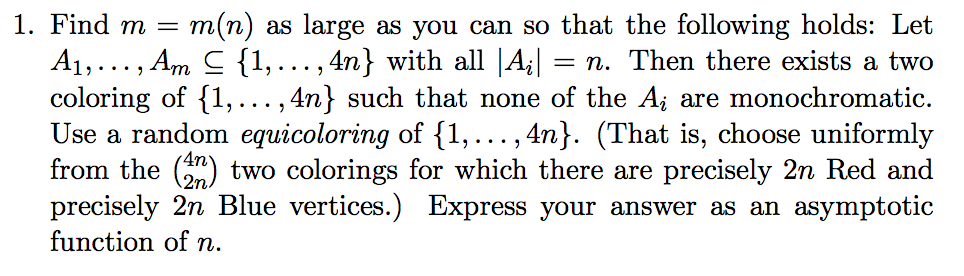
\includegraphics[width=1\textwidth]{pm-1-1.png}
\end{figure}
\end{question}
\begin{solution}
\end{solution}

\bigskip

\begin{question}[2]
\hfill
\begin{figure}[h!]
  \centering
    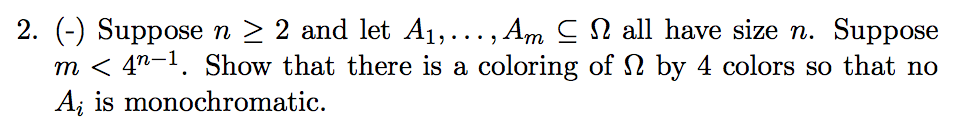
\includegraphics[width=1\textwidth]{pm-1-2.png}
\end{figure}
\end{question}
\begin{solution}
\textbf{(a)}
Let $x \in \text{Int} A \cup \text{Int} B$. It follows that there exists a neighborhood of 
$x$ contained in $A$ or exists a neighborhood of $x$ contained in $B$, respectively denoted 
as $U_A$ and $U_B$. If we have the existence of $U_A$, it follows that 
$x \in U_A \subset A \subset A \cup B$. Likewise, if we have the existence of $U_B$, it follows
that $x \in U_B \subset B \subset A \cup B$. Therefore, we have $x$ is an interior point of $A
\cup B$.
Since $x$ was arbitrary, we have shown that $\text{Int} A \cup \text{Int} B 
\subset \text{Int}(A \cup B)$. We now show that the equality does not hold, by providing
a counter example. Let $A = \mathbb{Q}$, $B = \mathbb{R\setminus Q}$. Then, 
$\text{int}\mathbb{R} = \mathbb{R}$ and $\text{int}\mathbb{Q} = \emptyset$ and 
$\text{int}\mathbb{R\setminus Q} = \emptyset$. Since $\mathbb{R} \not\subset
\emptyset$, we have shown that the equality does not hold. \hfill $\qed$  

\bigskip

\textbf{(b)}

 
\end{solution}

\bigskip

\begin{question}[3]
\hfill
\begin{figure}[h!]
  \centering
    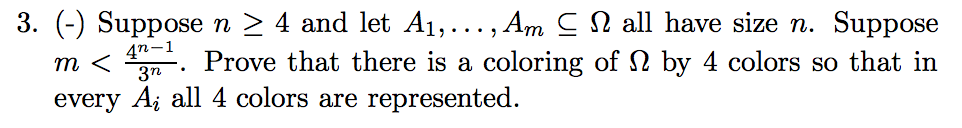
\includegraphics[width=1\textwidth]{pm-1-3.png}
\end{figure}
\end{question}
\begin{solution}
\end{solution}
\bigskip

\begin{question}[4]
\hfill
\begin{figure}[h!]
  \centering
    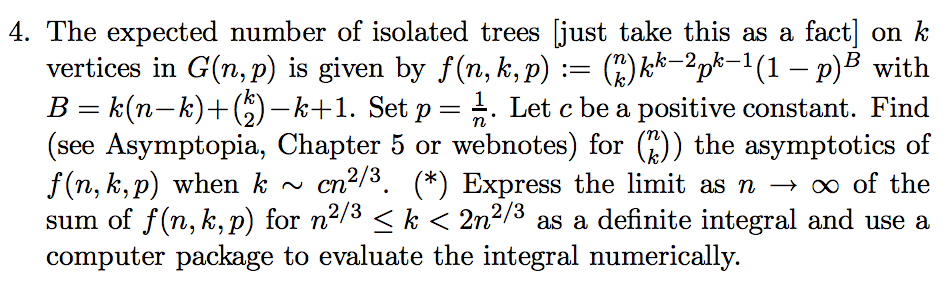
\includegraphics[width=1\textwidth]{pm-1-4.png}
\end{figure}
\end{question}
\begin{solution}
\end{solution}

\pagebreak

\begin{question}[5]
\hfill
\begin{figure}[h!]
  \centering
    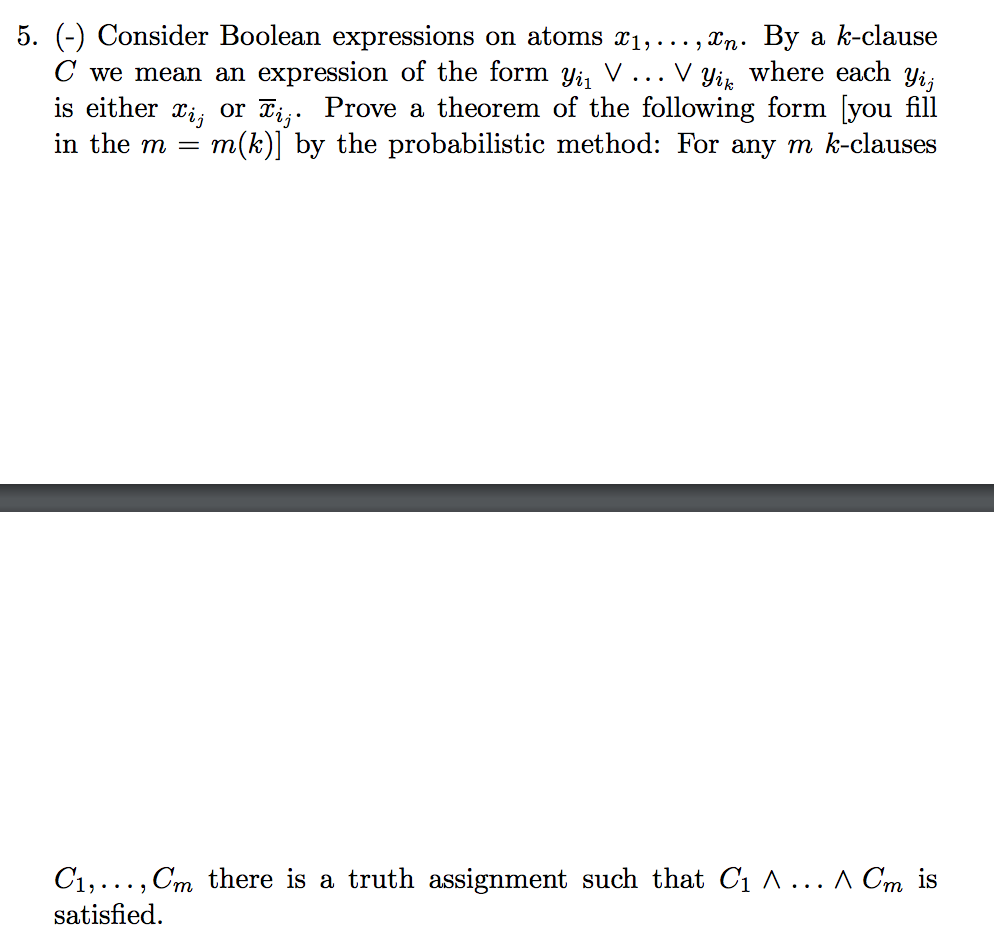
\includegraphics[width=1\textwidth]{pm-1-5.png}
\end{figure}
\end{question}
\begin{solution} 

 
\end{solution}

\pagebreak

\begin{question}[6]
\hfill
\begin{figure}[h!]
  \centering
    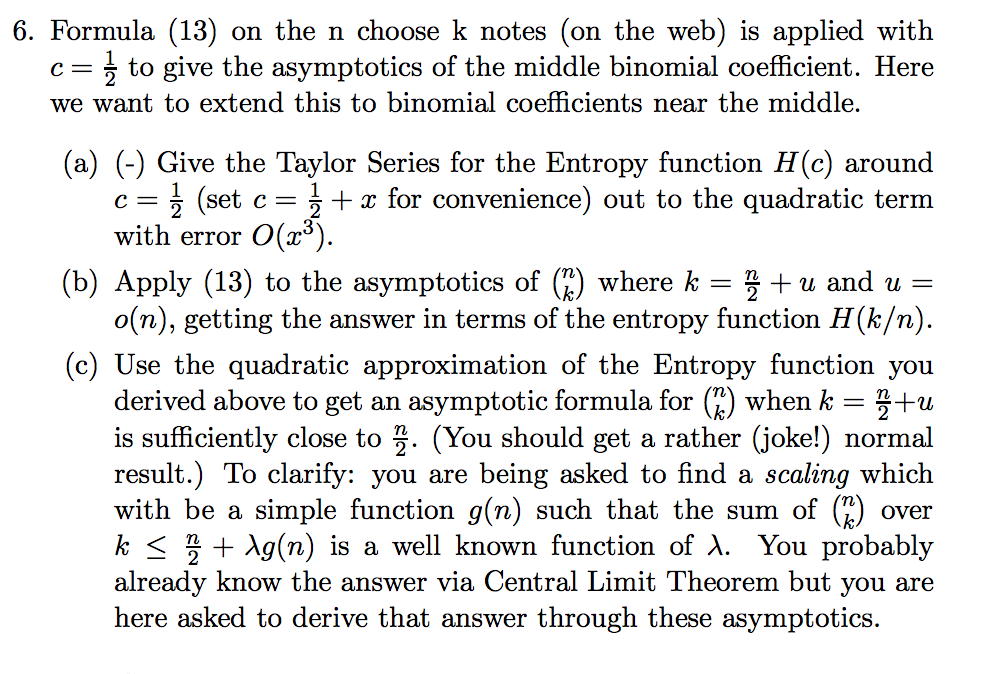
\includegraphics[width=1\textwidth]{pm-1-6.png}
\end{figure}
\end{question}
\begin{solution} 

 
\end{solution}
\end{document}
